% 1977 年湖南株洲卷第 9（2）题：菱形 ABCD（A 左、D 上、C 右、B 下），
% 对角线 BD 画虚线，A 处标 30°、B 处标 150°（按源卷第 4 页布局）
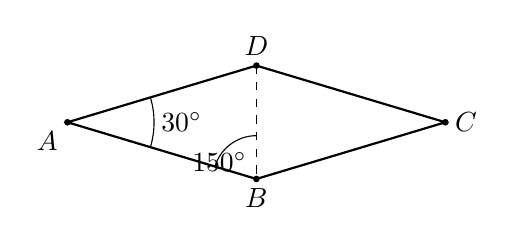
\begin{tikzpicture}[scale=1.0]
  \coordinate (A) at (0,0);
  \coordinate (D) at (2.4,0.72);
  \coordinate (C) at (4.8,0);
  \coordinate (B) at (2.4,-0.72);
  \draw[thick] (A)--(D)--(C)--(B)--cycle;
  \draw[dashed] (D)--(B);
  \draw ([shift=(16.7:1.1)]A) arc (16.7:-16.7:1.1);
  \node at (1.45,0) {$30^\circ$};
  \draw ([shift=(90:0.55)]B) arc (90:163.3:0.55);
  \node at (1.93,-0.50) {$150^\circ$};
  \fill (A) circle (1.2pt) node[below left] {$A$};
  \fill (B) circle (1.2pt) node[below] {$B$};
  \fill (C) circle (1.2pt) node[right] {$C$};
  \fill (D) circle (1.2pt) node[above] {$D$};
\end{tikzpicture}
